\documentclass[12pt, a4paper, oneside]{article}
\usepackage{graphicx}
\usepackage{arial}
\renewcommand{\familydefault}{\sfdefault}
\usepackage[T1]{fontenc}
\usepackage[polish]{babel}
\usepackage[utf8]{inputenc}
\usepackage{lmodern}
\usepackage[left=2cm,right=2cm,top=2cm,bottom=2cm]{geometry}
\selectlanguage{polish}

\begin{document}
\pagenumbering{gobble}
\pagenumbering{arabic}
\section{Wstęp}
\indent\indent Proces spawania światłowodów ma na celu połączenie dwóch włókien na stałe przy zachowaniu małego tłumienia wykonanego połączenia. Typowe tłumienie poprawnie wykonanego spawu jest zazwyczaj mniejsze niż 0.2 dB. Tłumienie to można sprawdzić na kilka sposobów. Najmniej dokładnym sposobem jest odczyt wartości wyznaczonej przez spawarkę. Należy ją jednak traktować jedynie poglądowo. Drugim sposobem jest wykonanie pomiarów reflektometrem przed spawaniem światłowodu, ustawienie markera w punkcie, gdzie światłowód ma swój koniec, a następnie wykonanie spawu i ponowny pomiar reflektometrem. W miejscu ustawionego markera teraz można zaobserwować straty odbiciowe wykonanego spawu. Podczas laboratorium tłumienie spawu wykonywane jest za pomocą pomiaru tłumienia odcinka. Znając długość łączną powstałego światłowodu oraz jego tłumienie w dB/km możemy określić tłumienie wykonanego spawu. Etapy procesu spawania:
\begin{itemize}
\item usunięcie powłoki lakierowanej za pomocą strippera,
\item wyczyszczenie odkrytego włókna izopropanolem,
\item prostopadłe przycięcie końcówki włókna,
\item umieszczenie włókien przeznaczonych do spawania w spawarce,
\item wykonanie prespawu w celu oczyszczenia końcówek włókien,
\item dosunięcie włókien na minimalny odstęp i dokładne wycentrowanie,
\item wykonanie właściwego spawu.
\begin{figure}[h]
\centering
\caption{Efekt przypadkowego uruchomienia spawania na bardzo rozsuniętych włóknach}
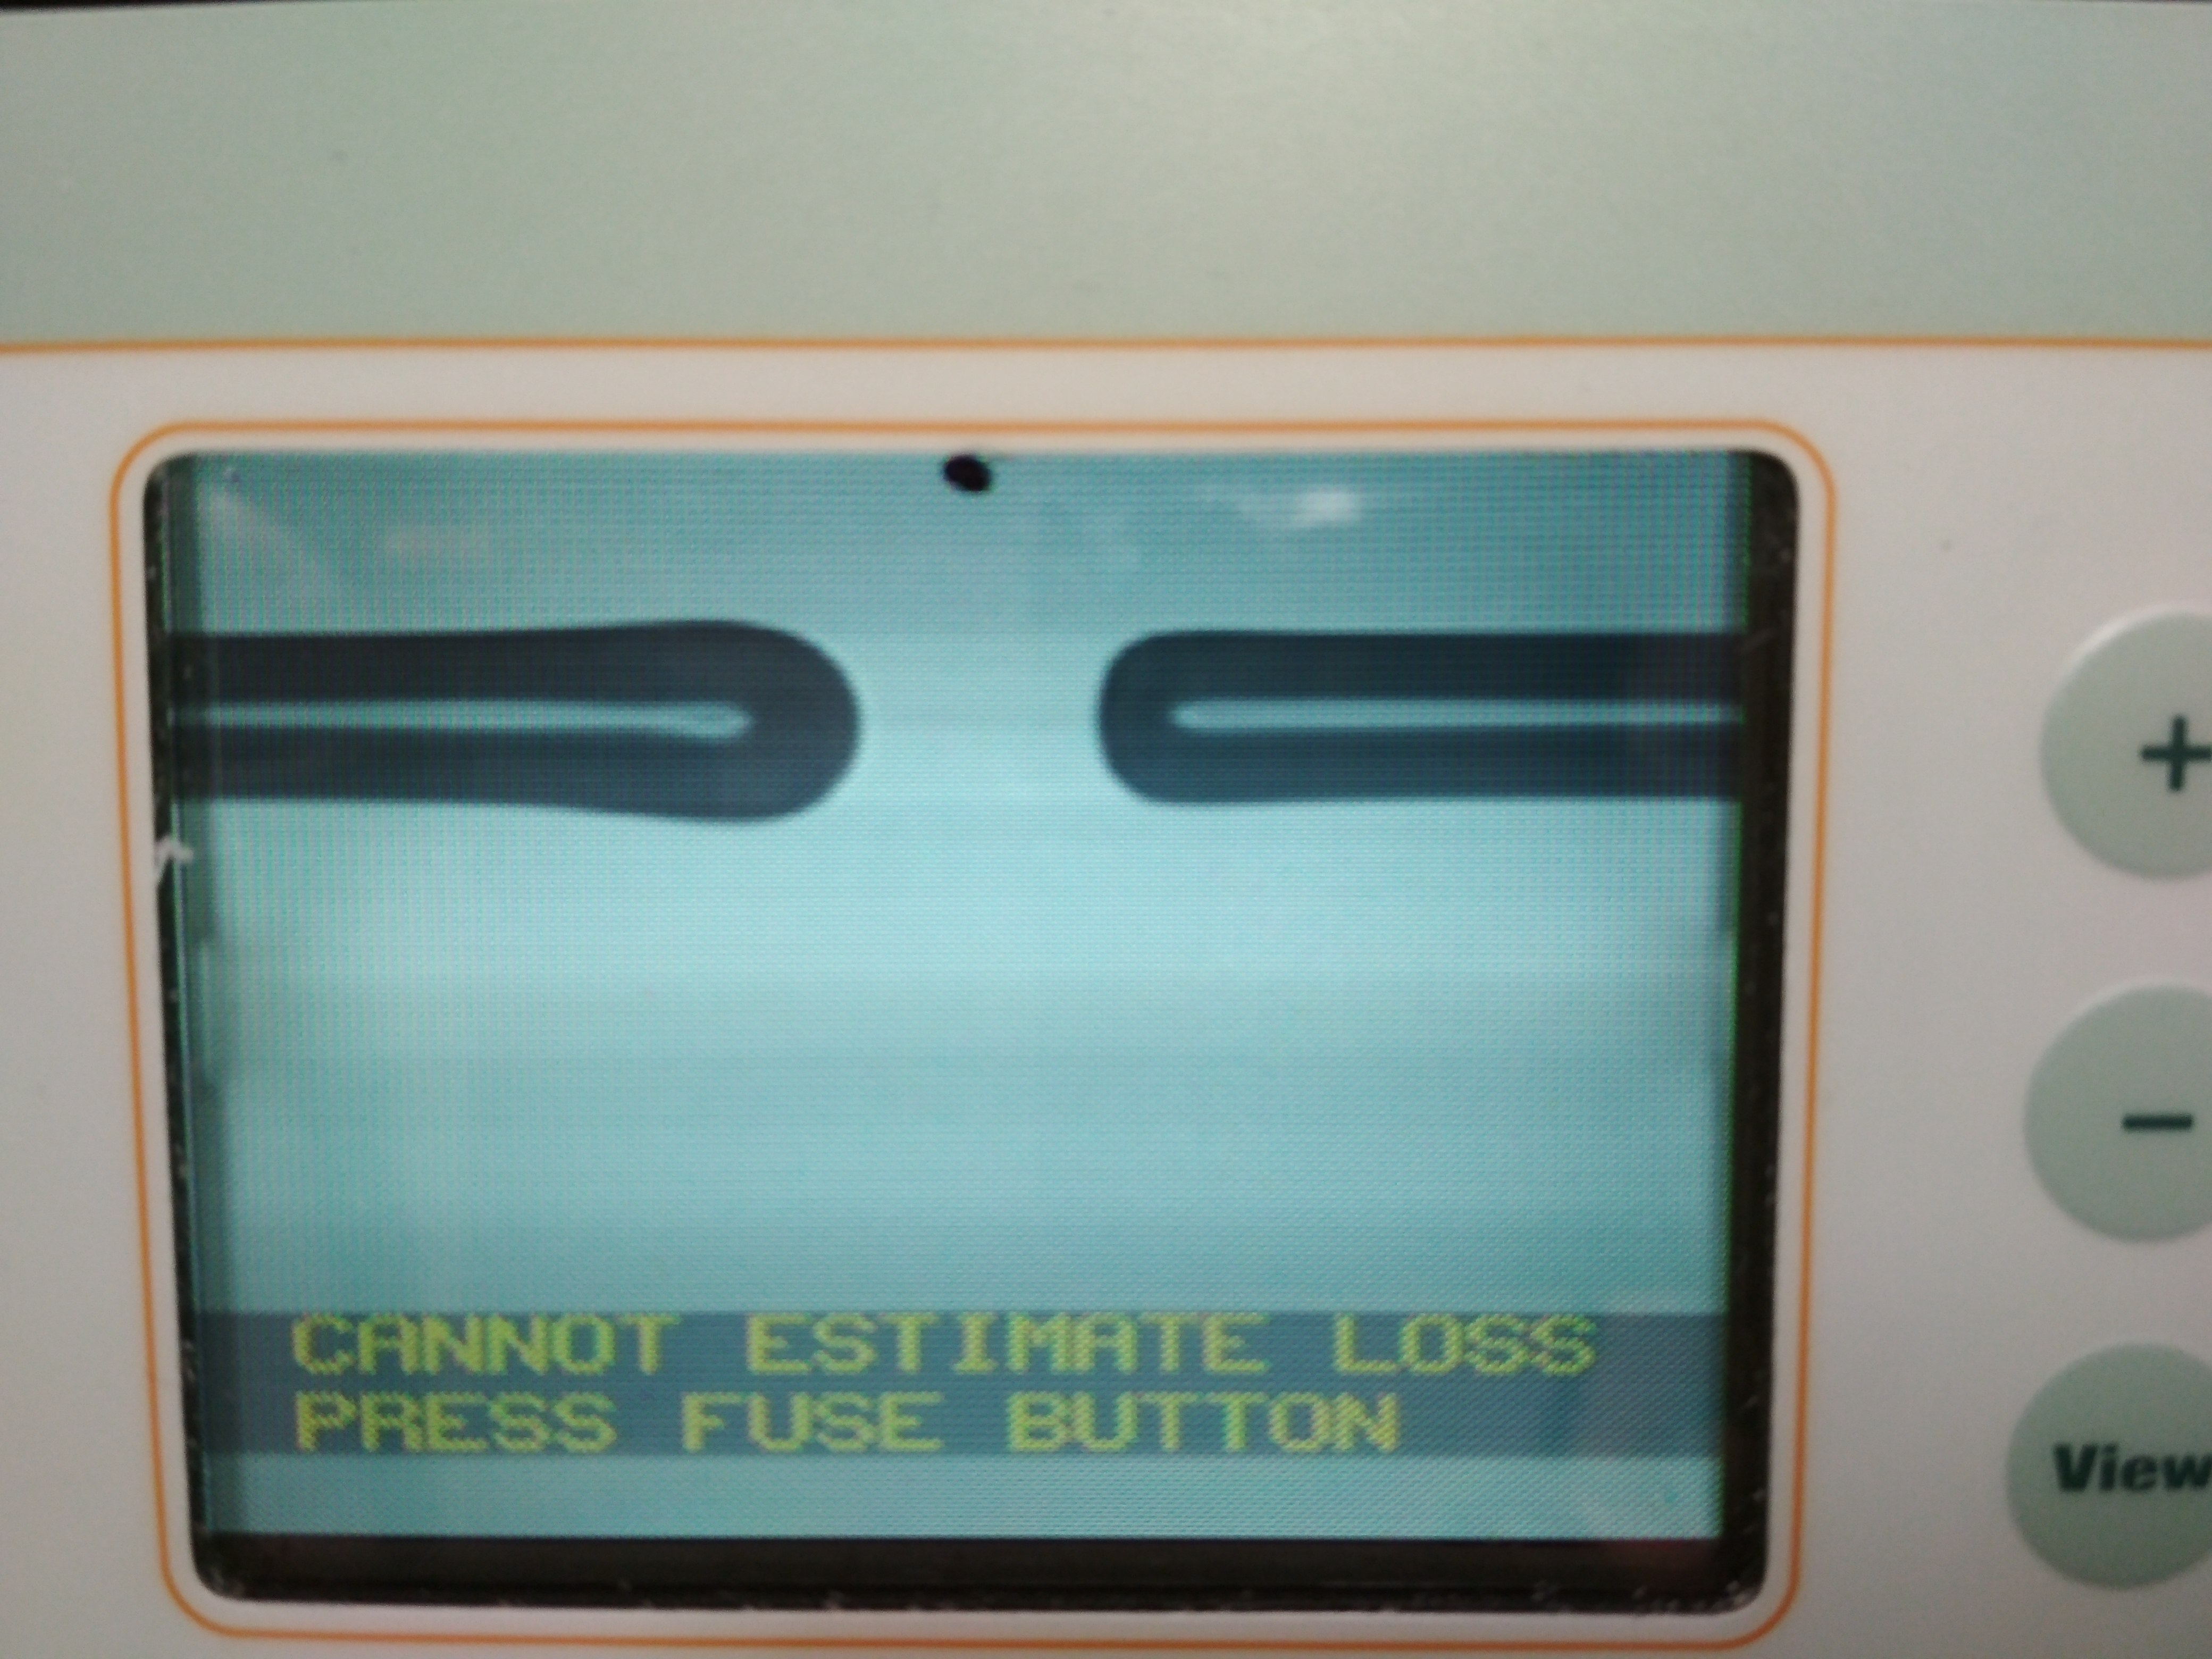
\includegraphics[scale=0.075]{f7.jpg}
\end{figure}
\end{itemize}
\clearpage
\section{Przebieg ćwiczenia}
\begin{figure}[h]
\centering
\caption{Oczyszczone i odpowiednio ucięte włókna światłowodowe przygotowane do prespawu}
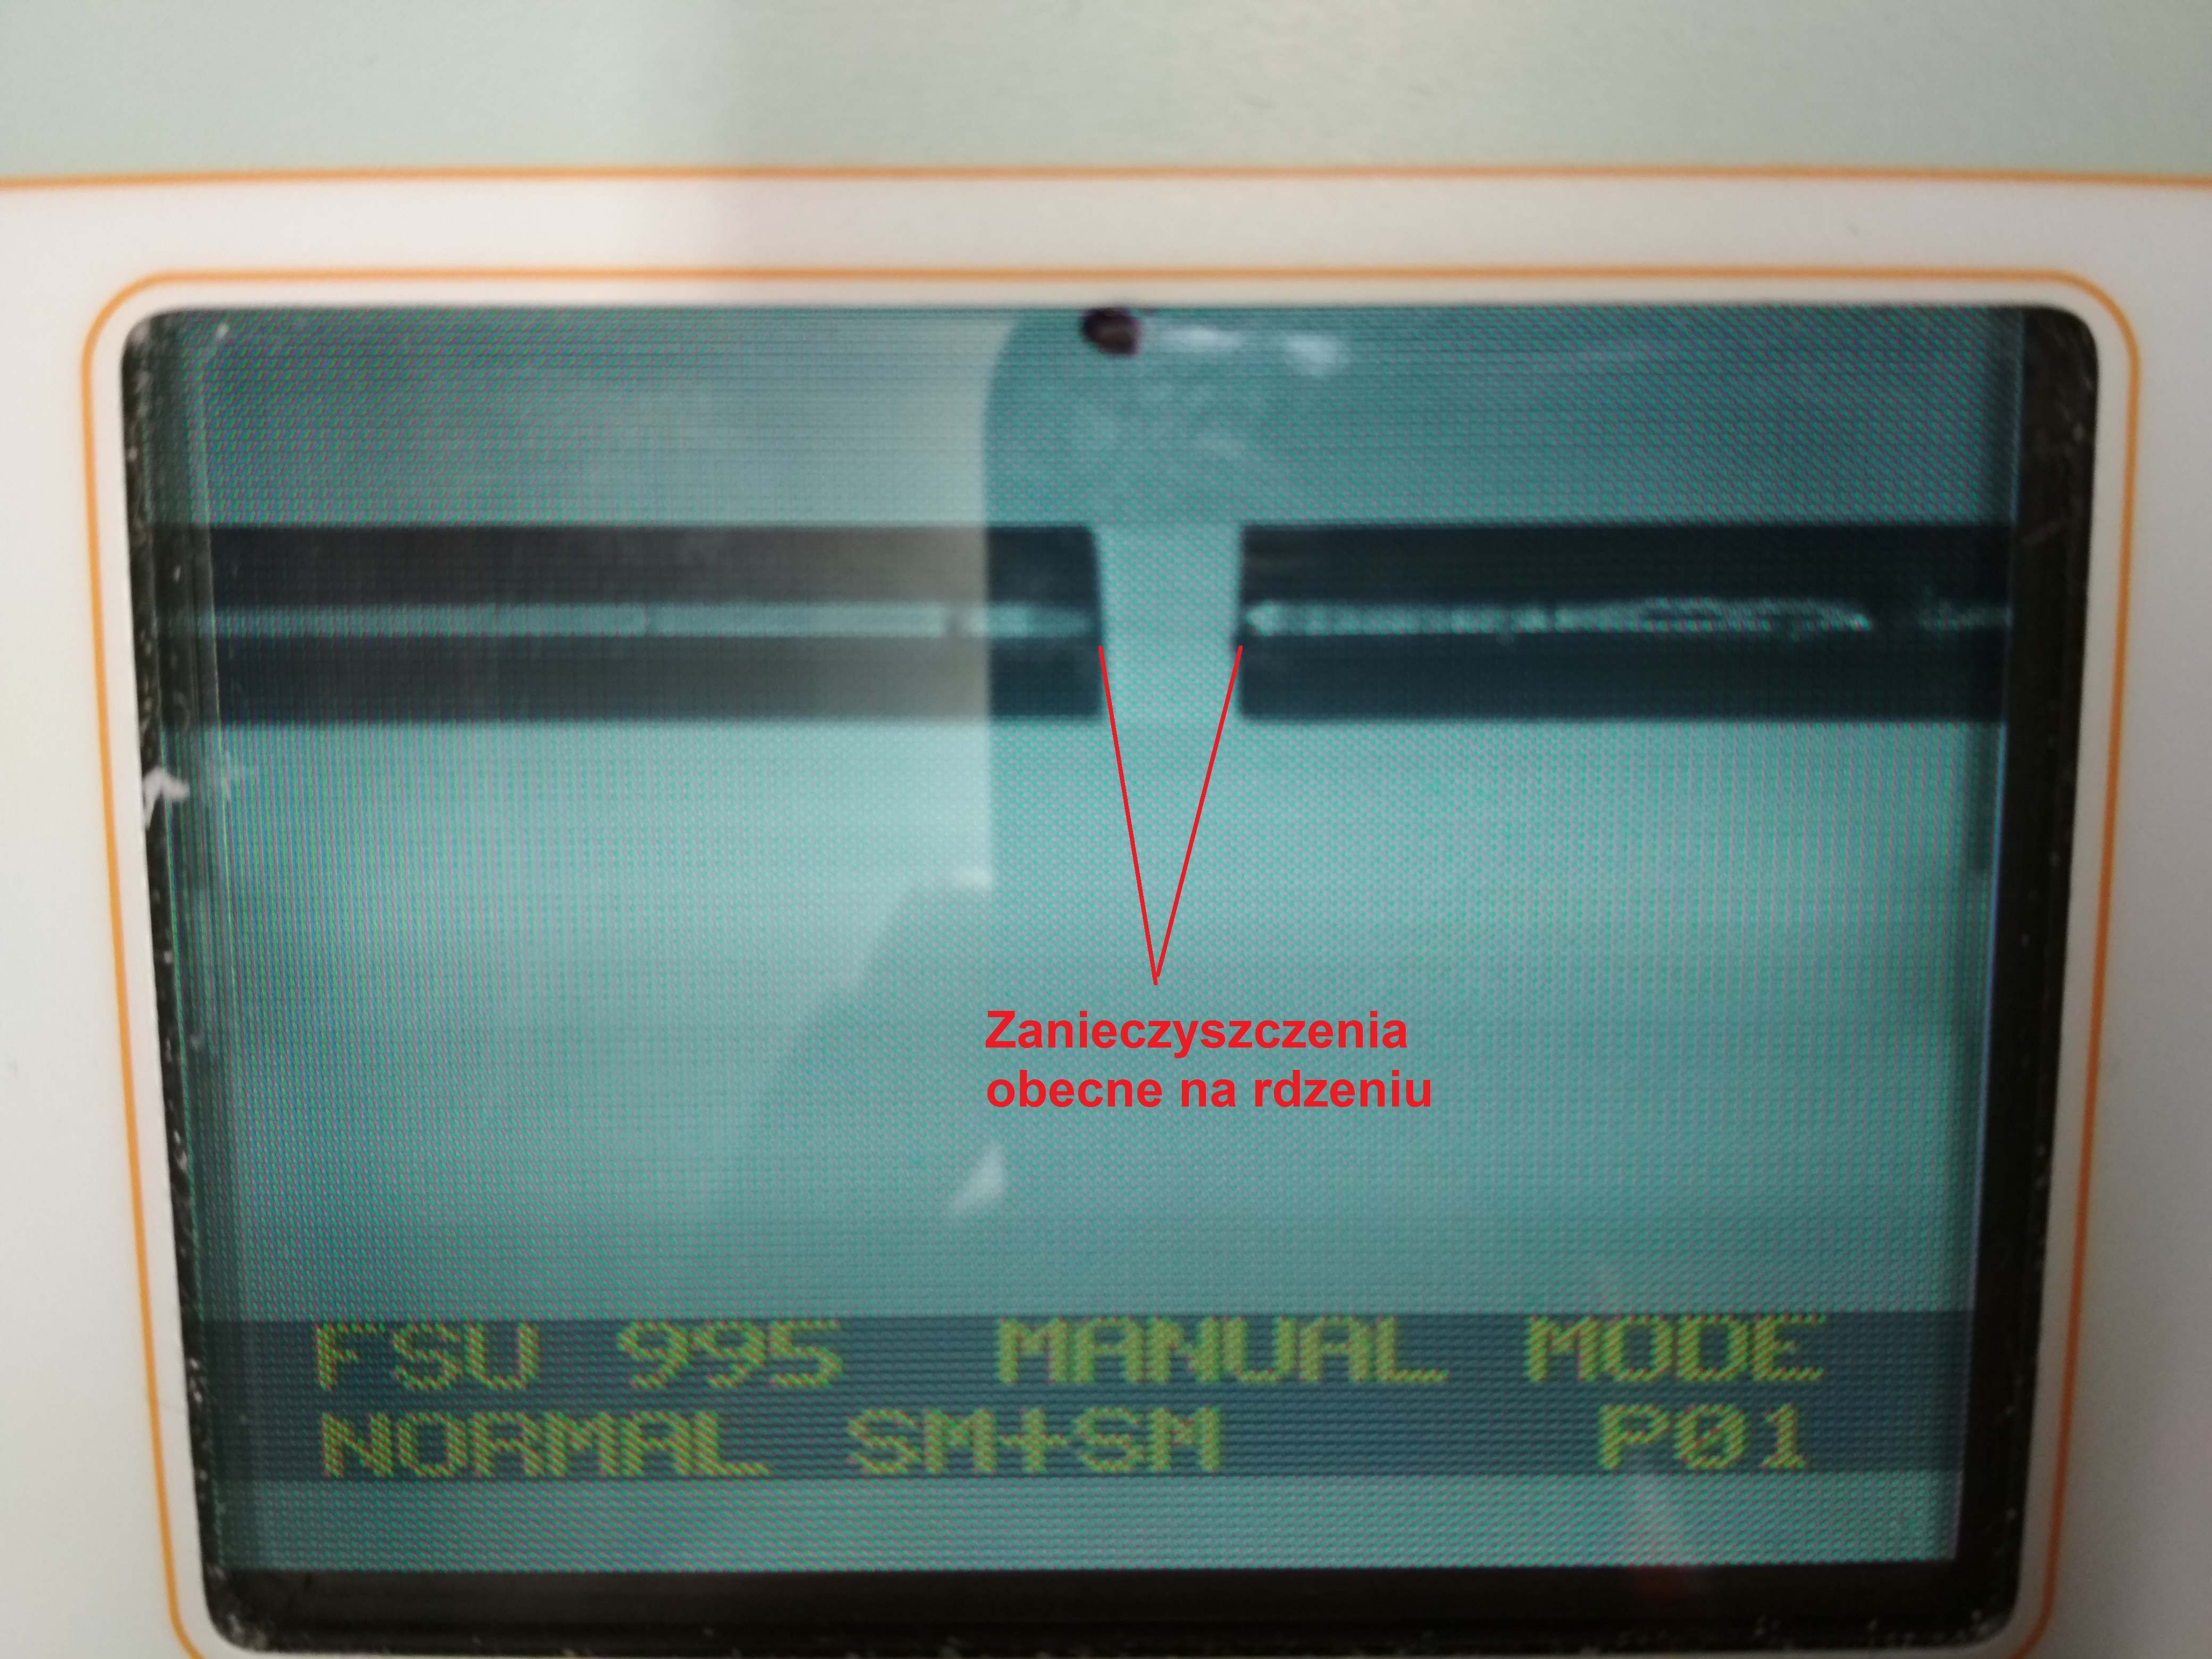
\includegraphics[scale=0.075]{f1.jpg}
\end{figure}\bigskip\bigskip\bigskip\bigskip\bigskip
\begin{figure}[h]
\centering
\caption{Włókna po wykonaniu prespawu}
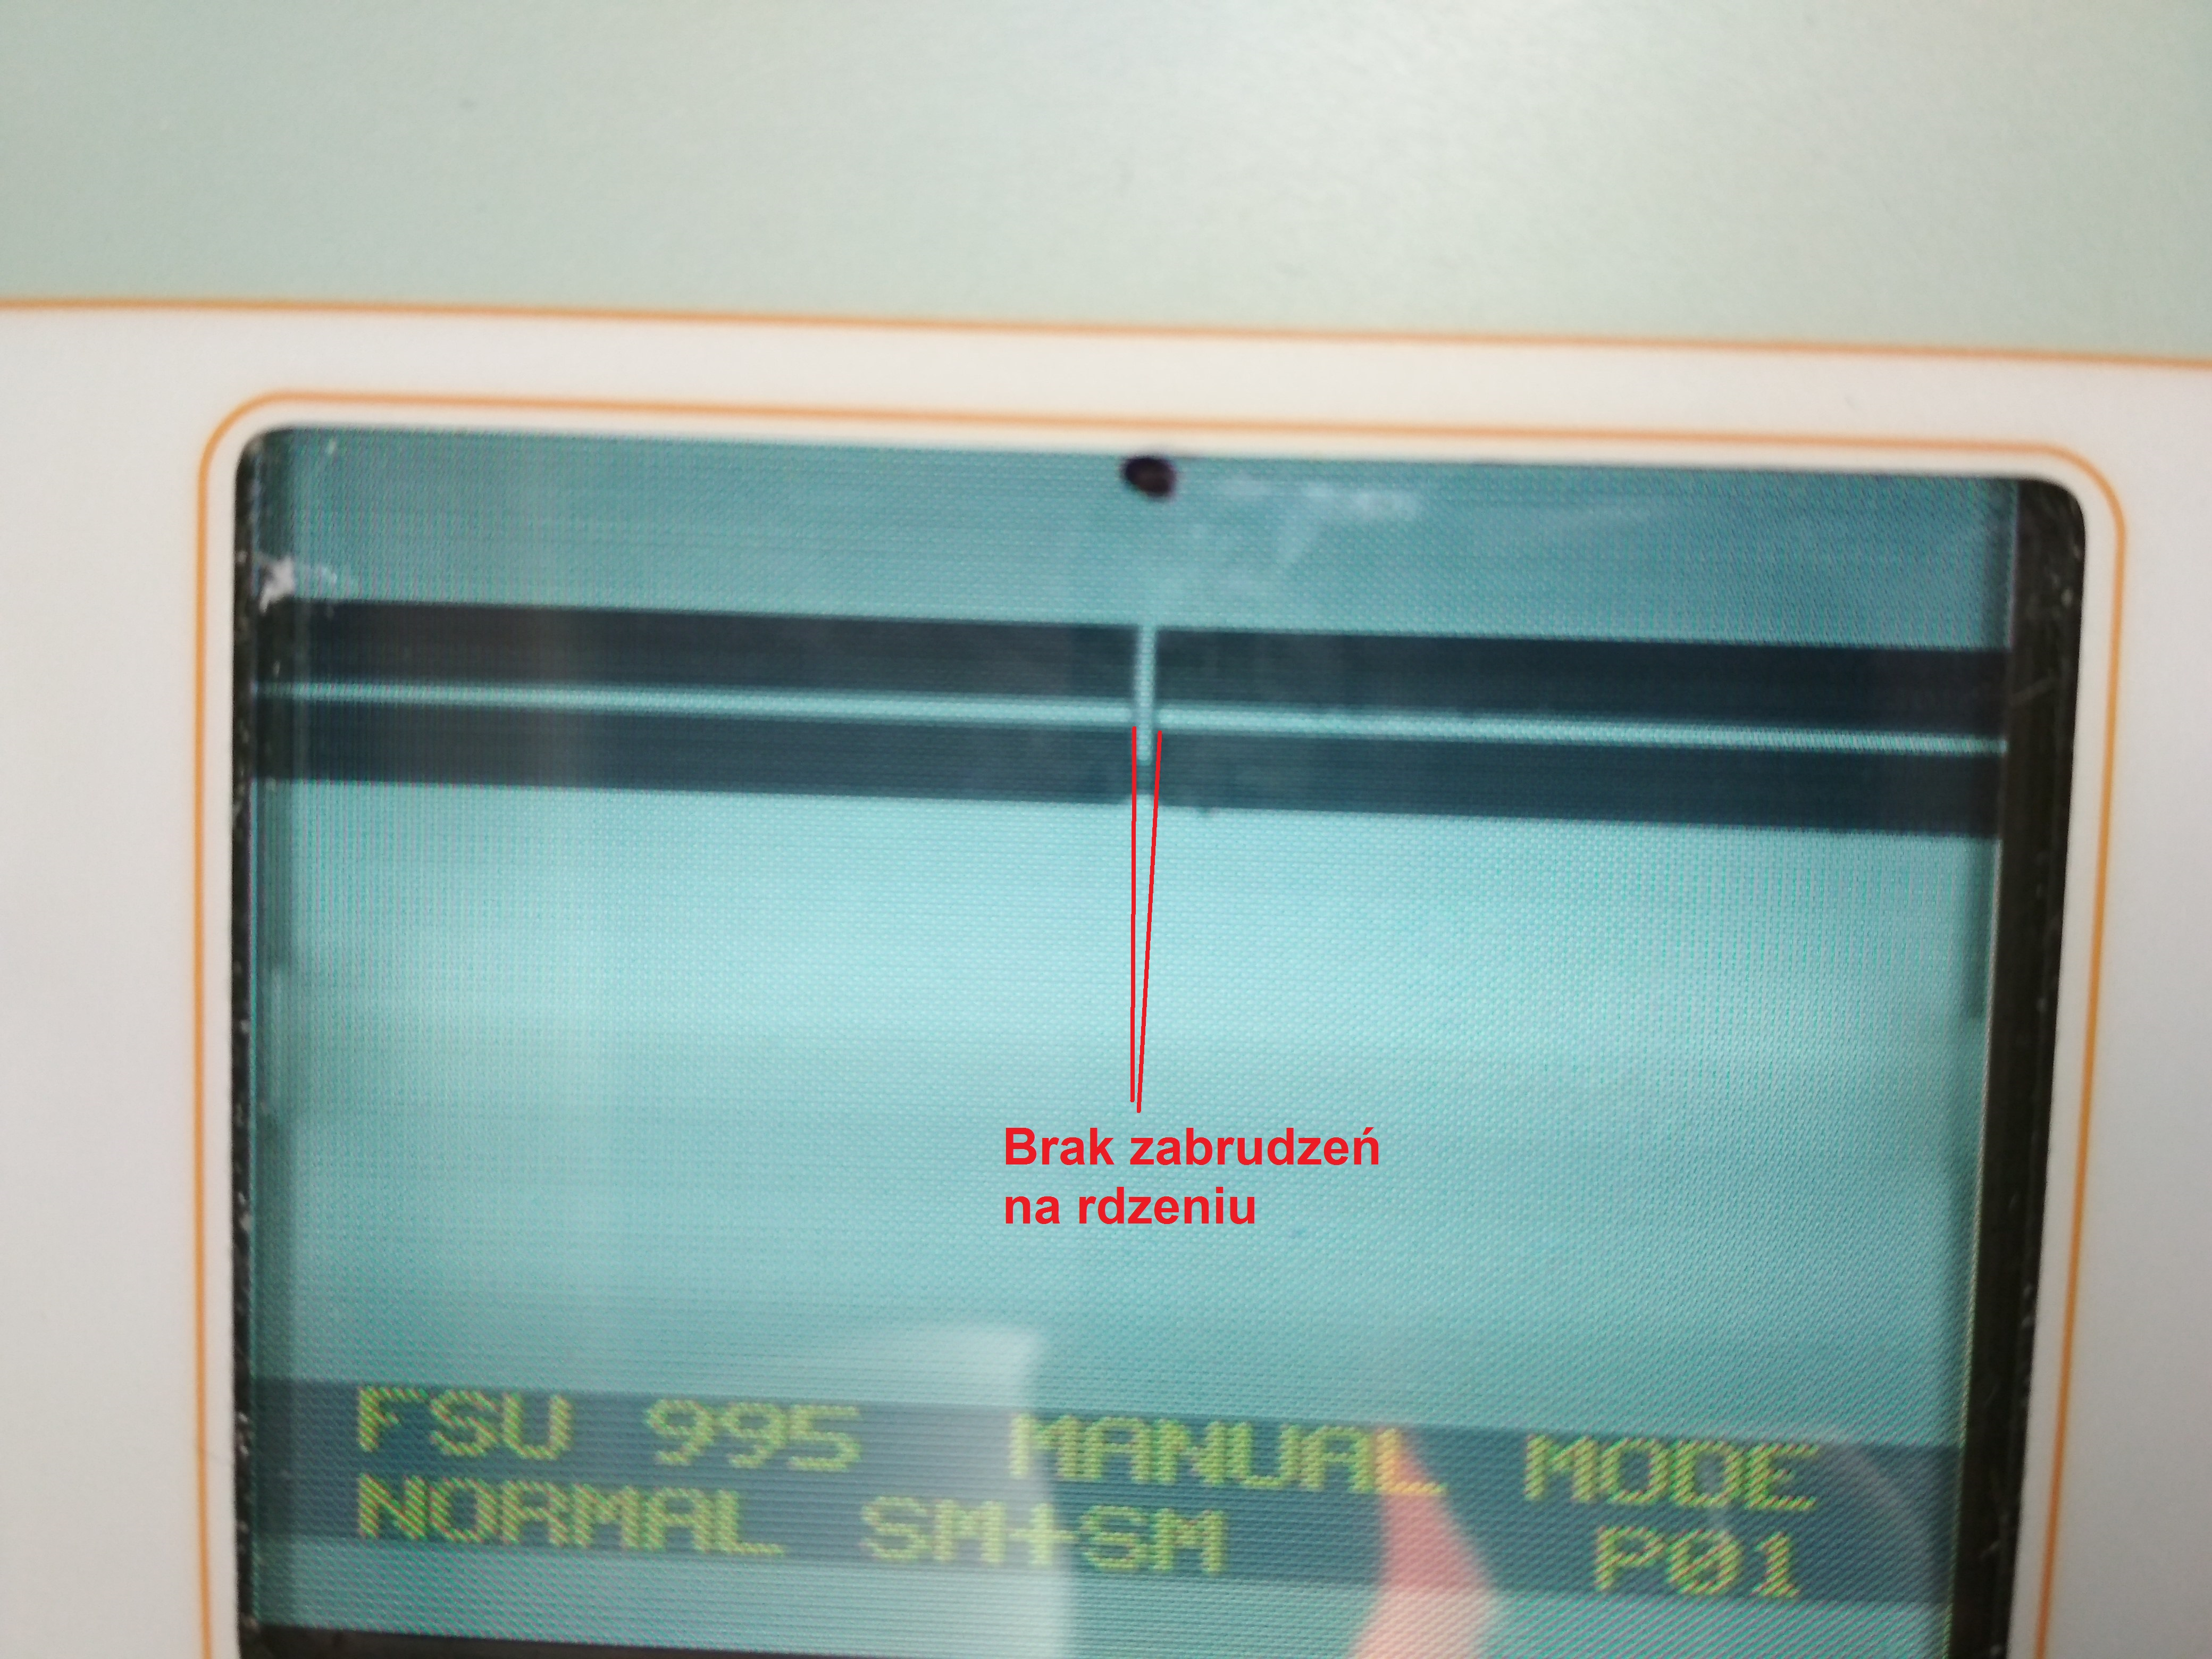
\includegraphics[scale=0.075]{f2.jpg}
\end{figure}
\clearpage
\begin{figure}[t]
\centering
\caption{Zdjęcie procesu spawania, podczas pracy elektrody}
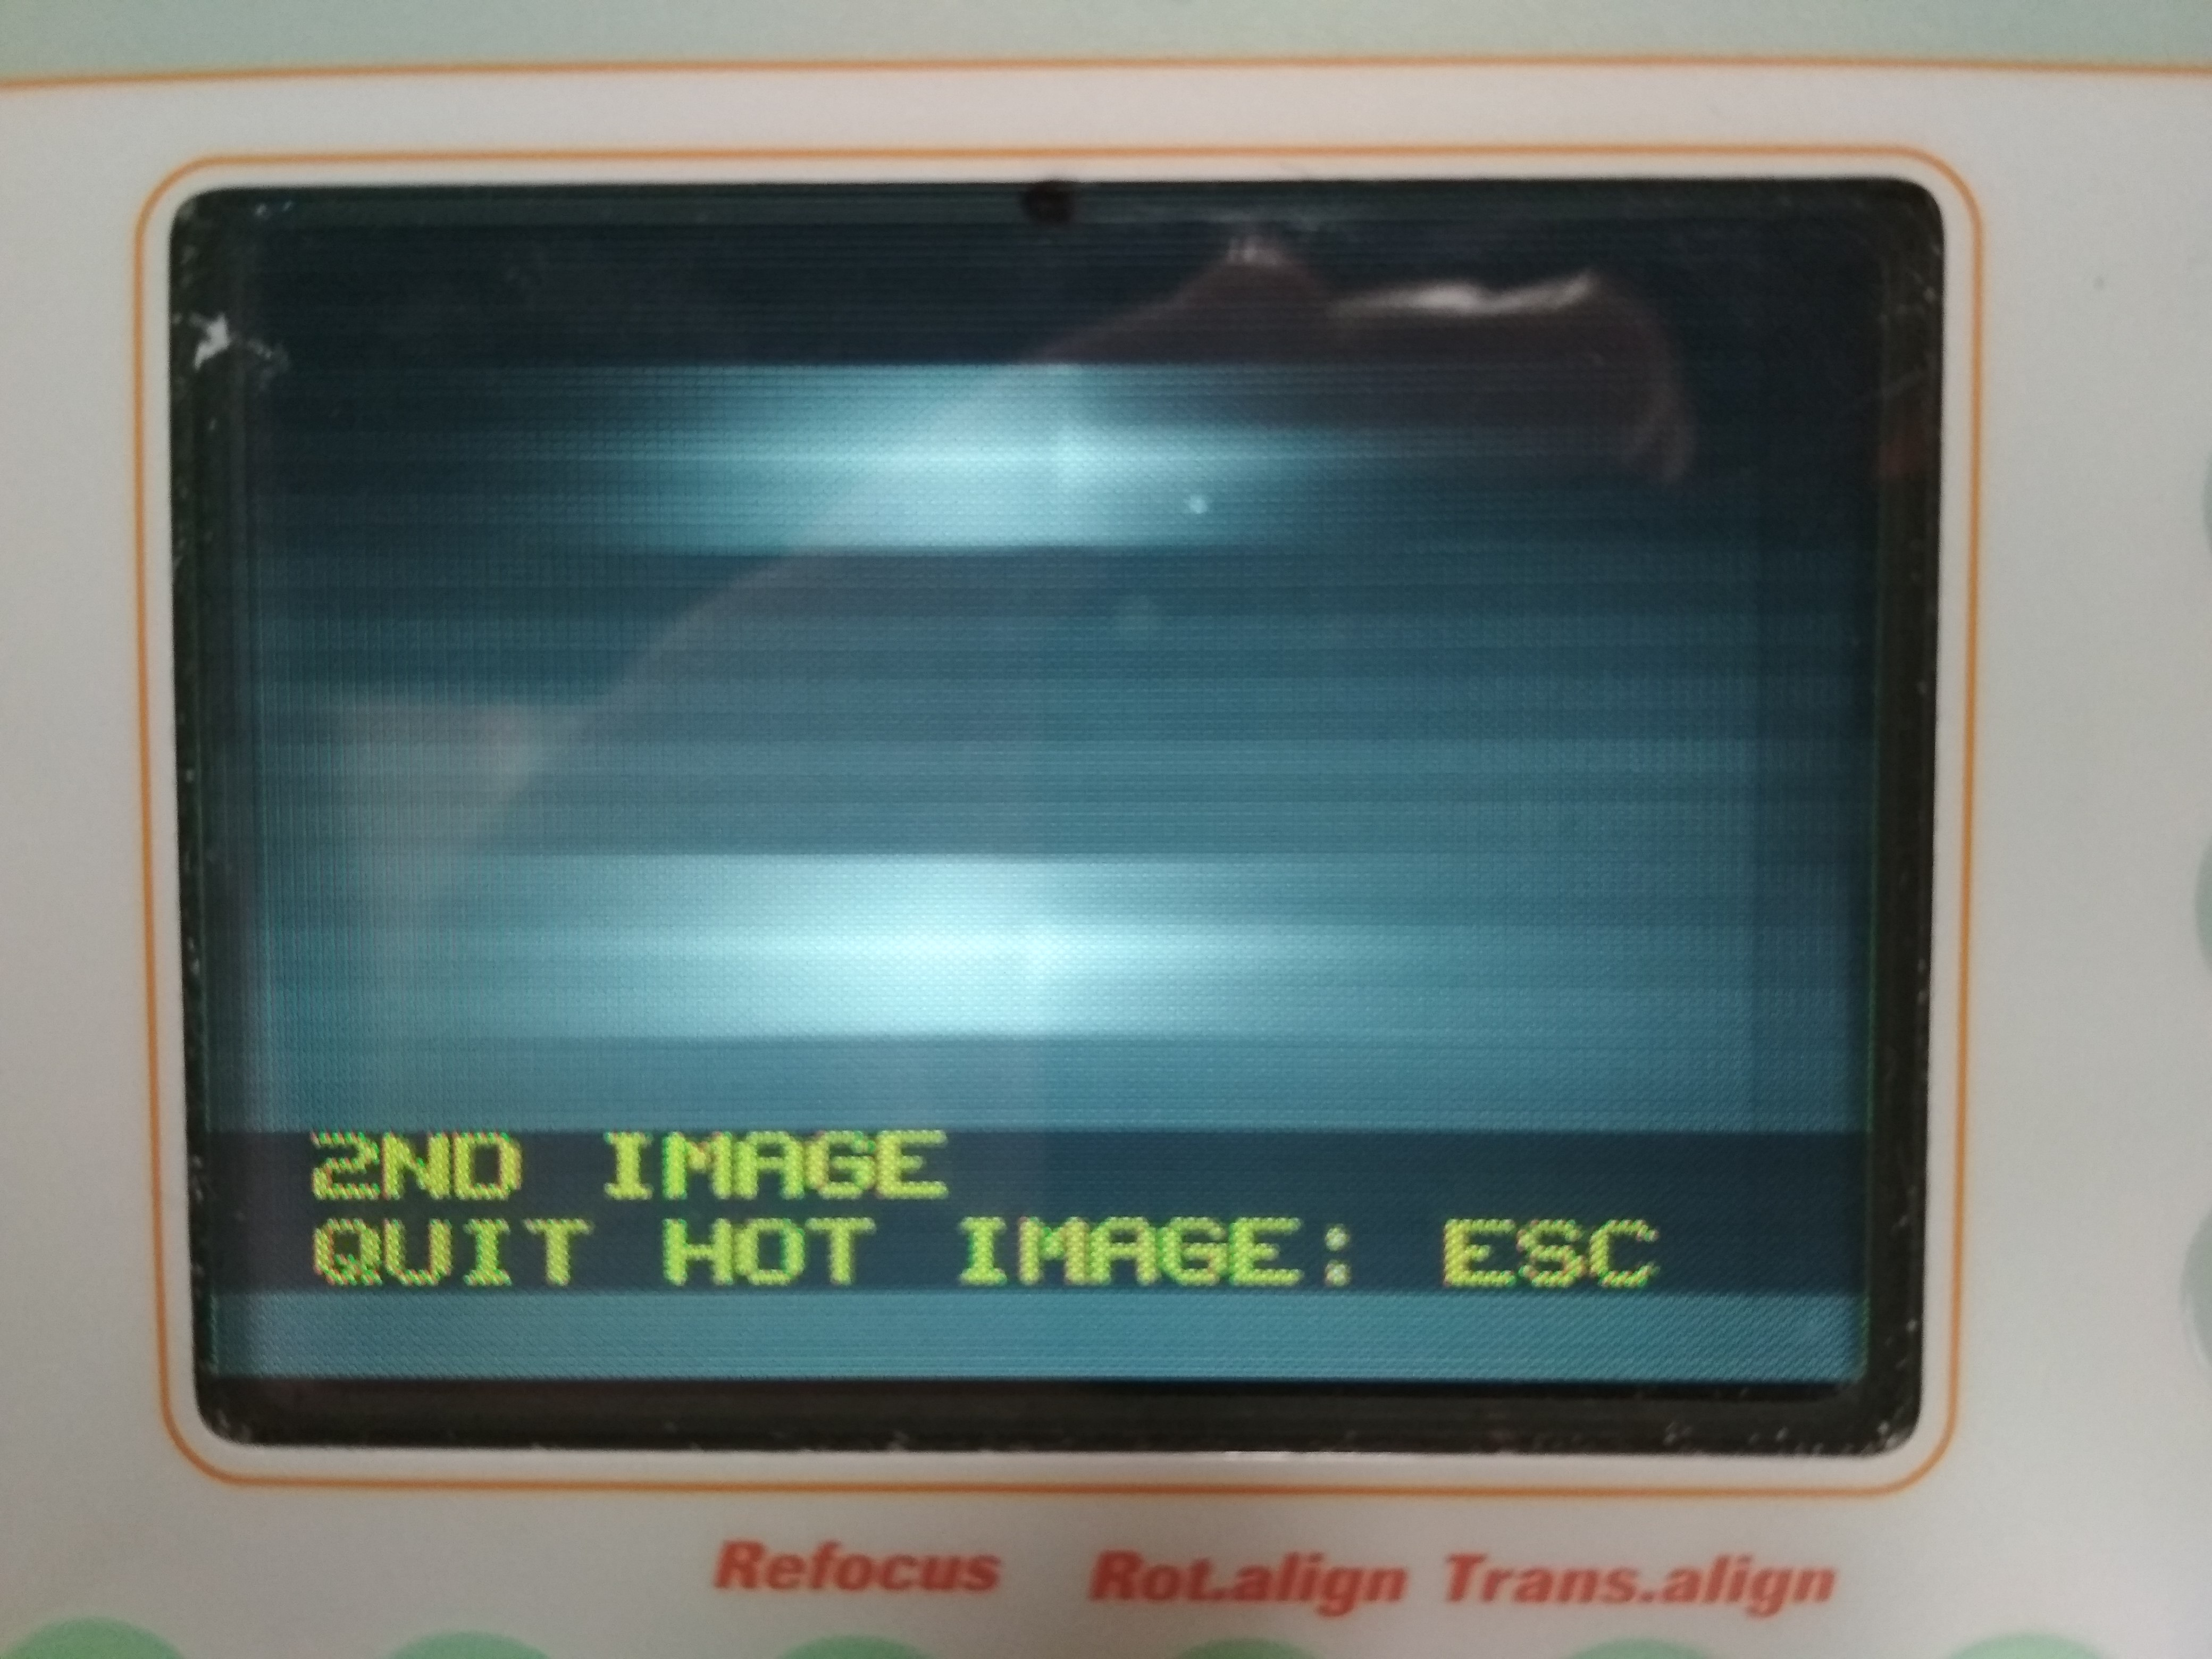
\includegraphics[scale=0.075]{f3.jpg}
\end{figure}
\begin{figure}[b]
\centering
\caption{Włókno po wykonaniu spawu}
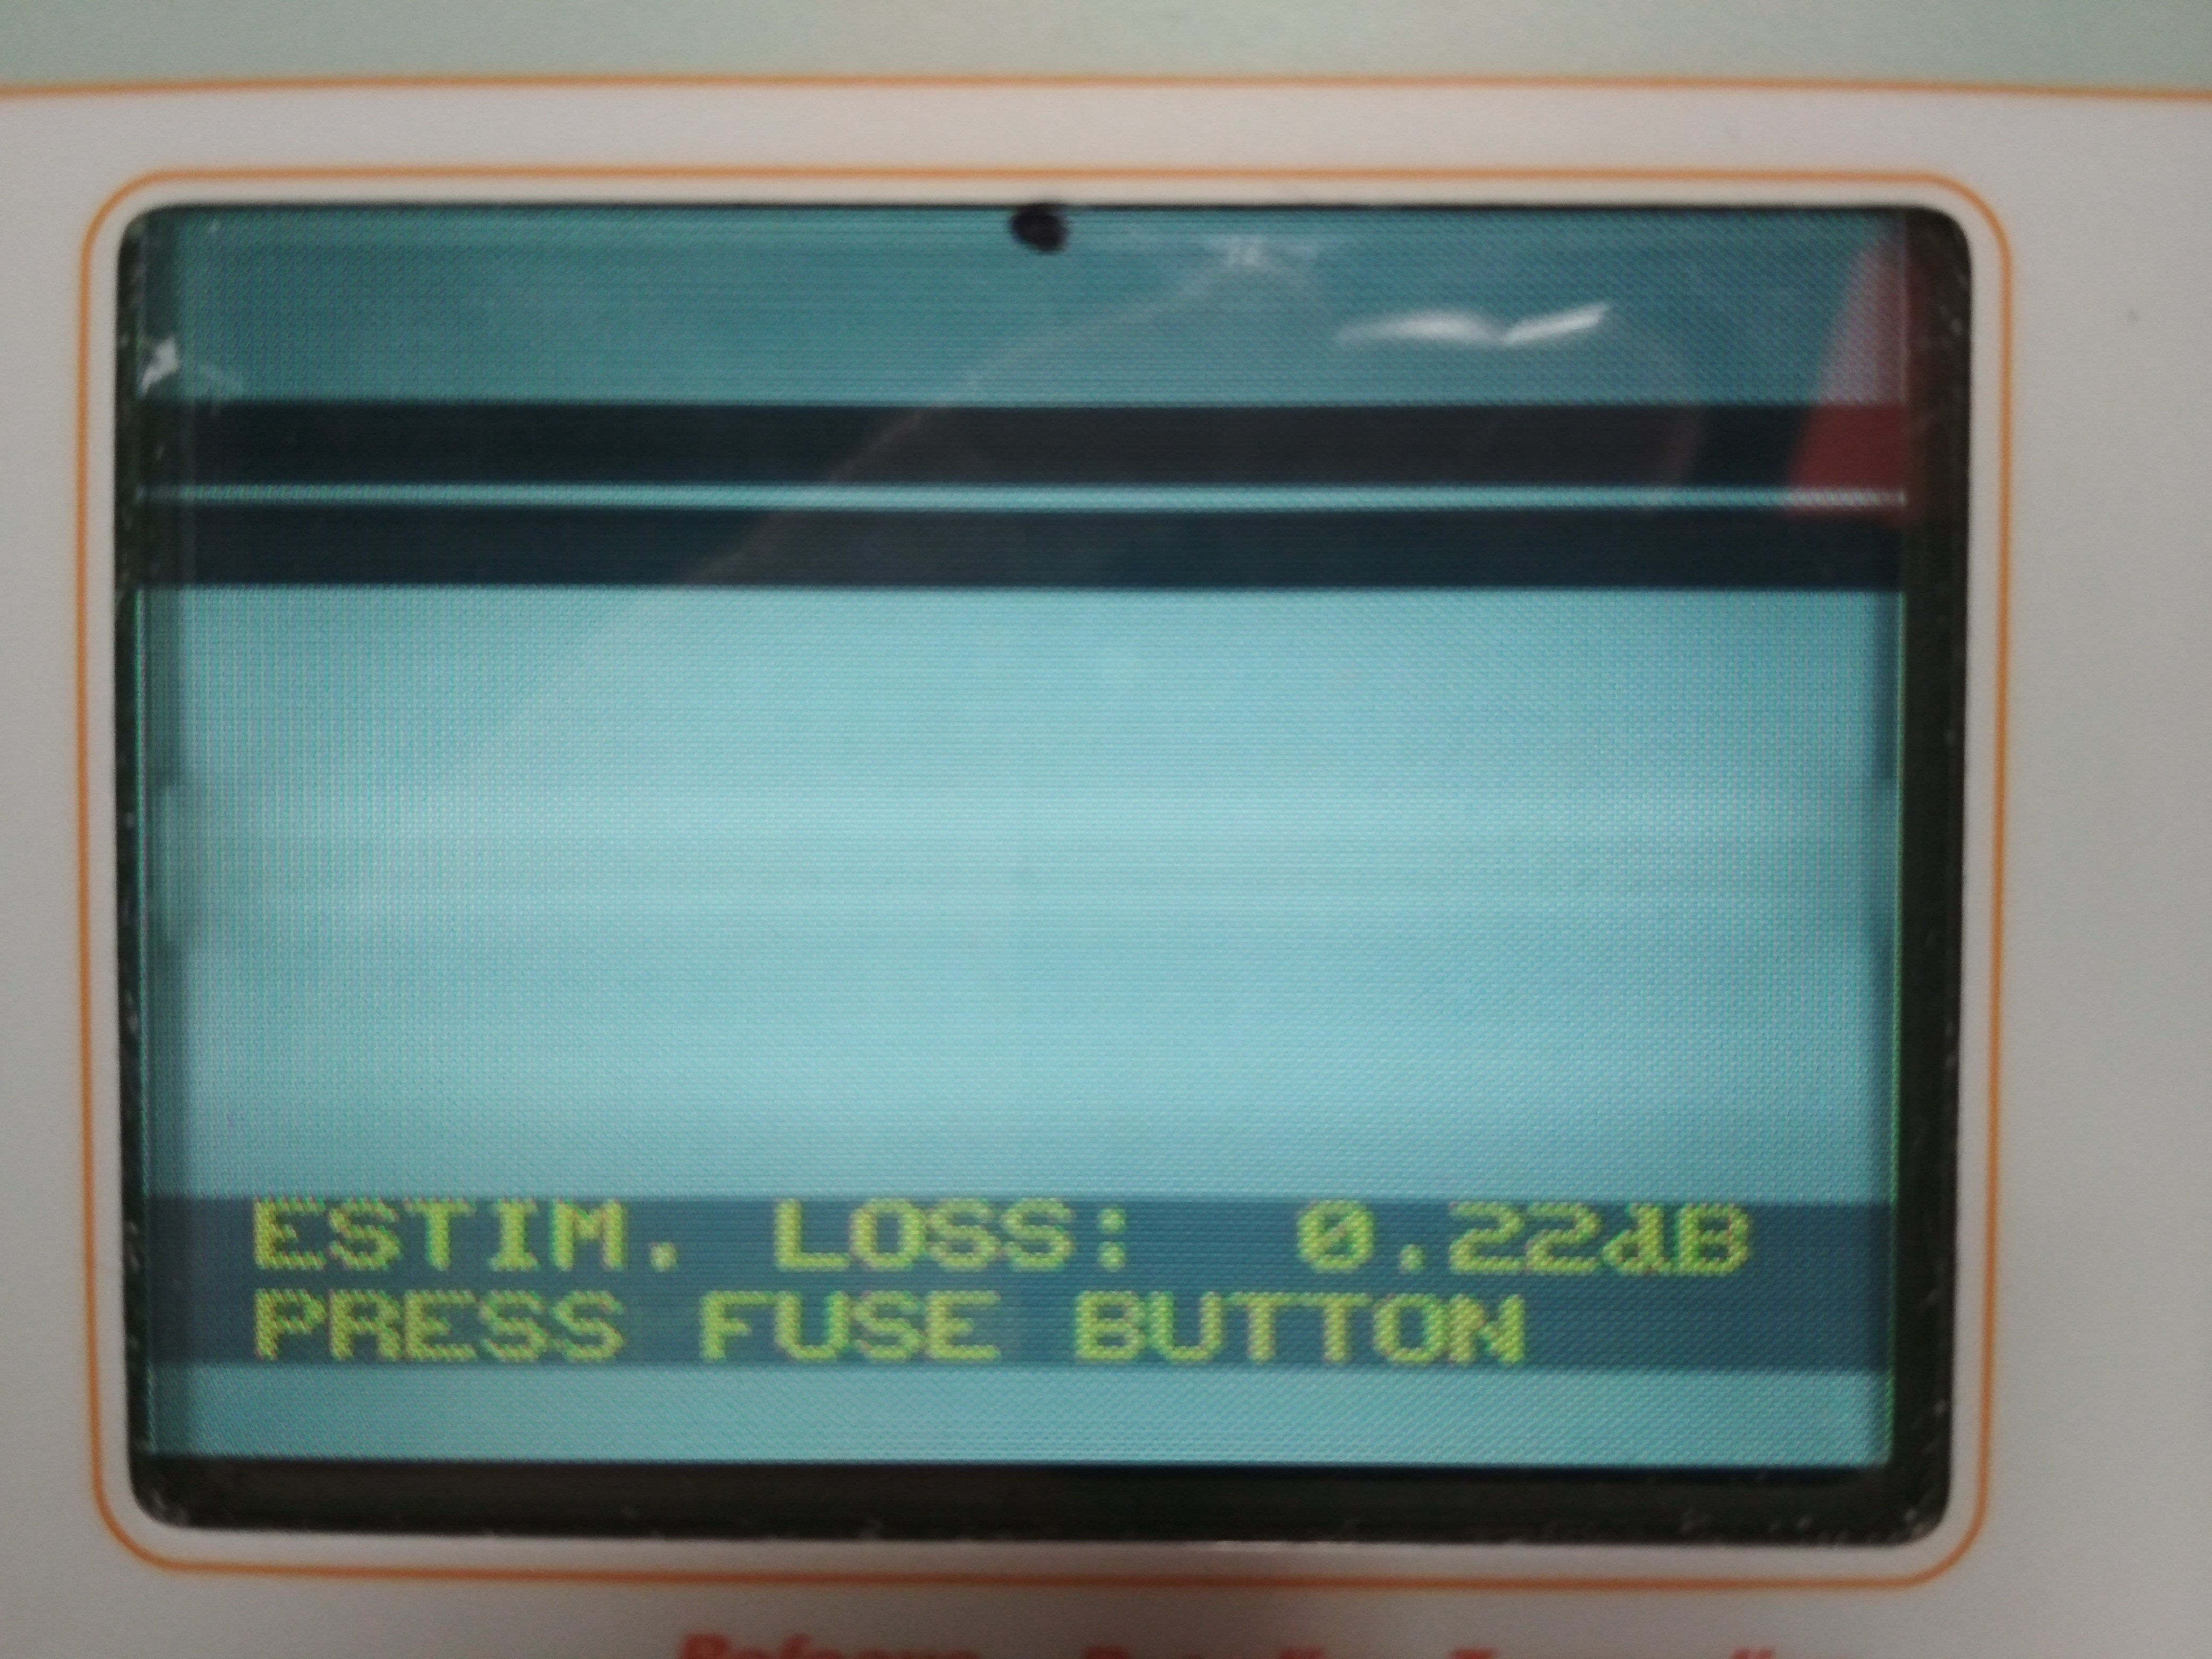
\includegraphics[scale=0.075]{f4.jpg}
\end{figure}
\clearpage
\begin{figure}[b]
\centering
\caption{Krzywe 3D przedstawiające intensywność światła we włóknie}
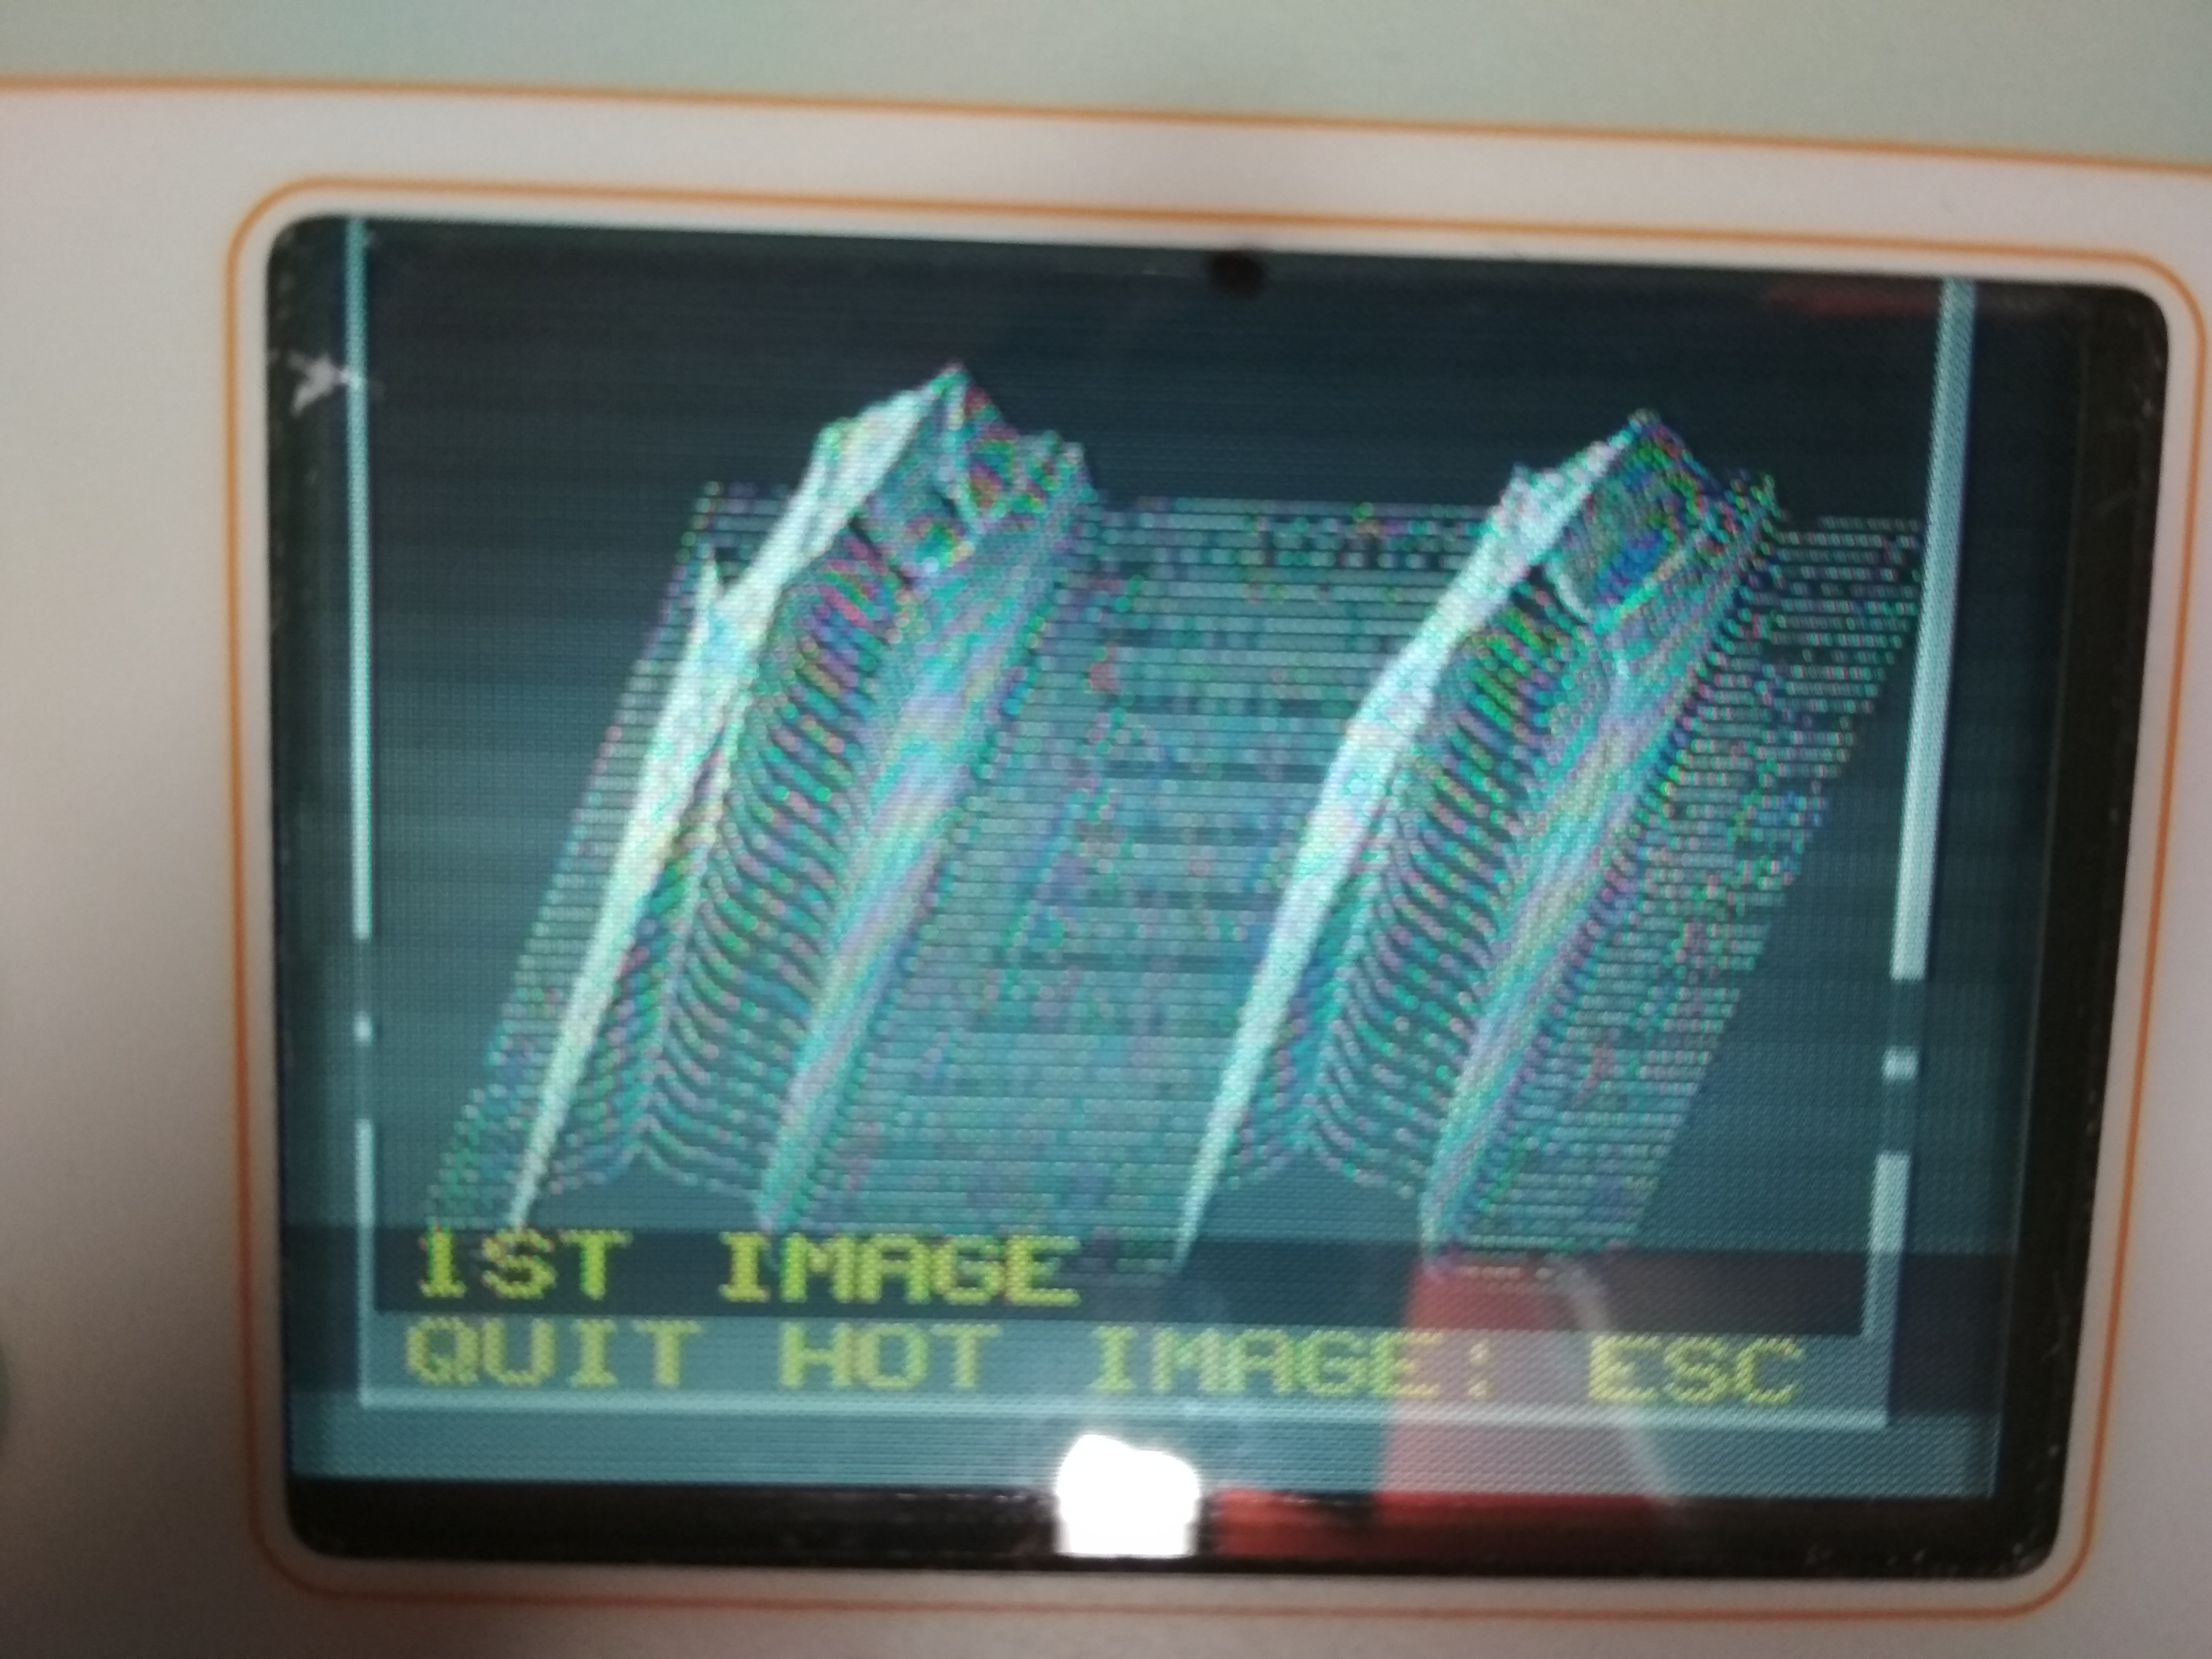
\includegraphics[scale=0.075]{f5.jpg}
\end{figure}
\begin{figure}[t]
\centering
\caption{Pomiar tłumienia w zespawanych światłowodach}
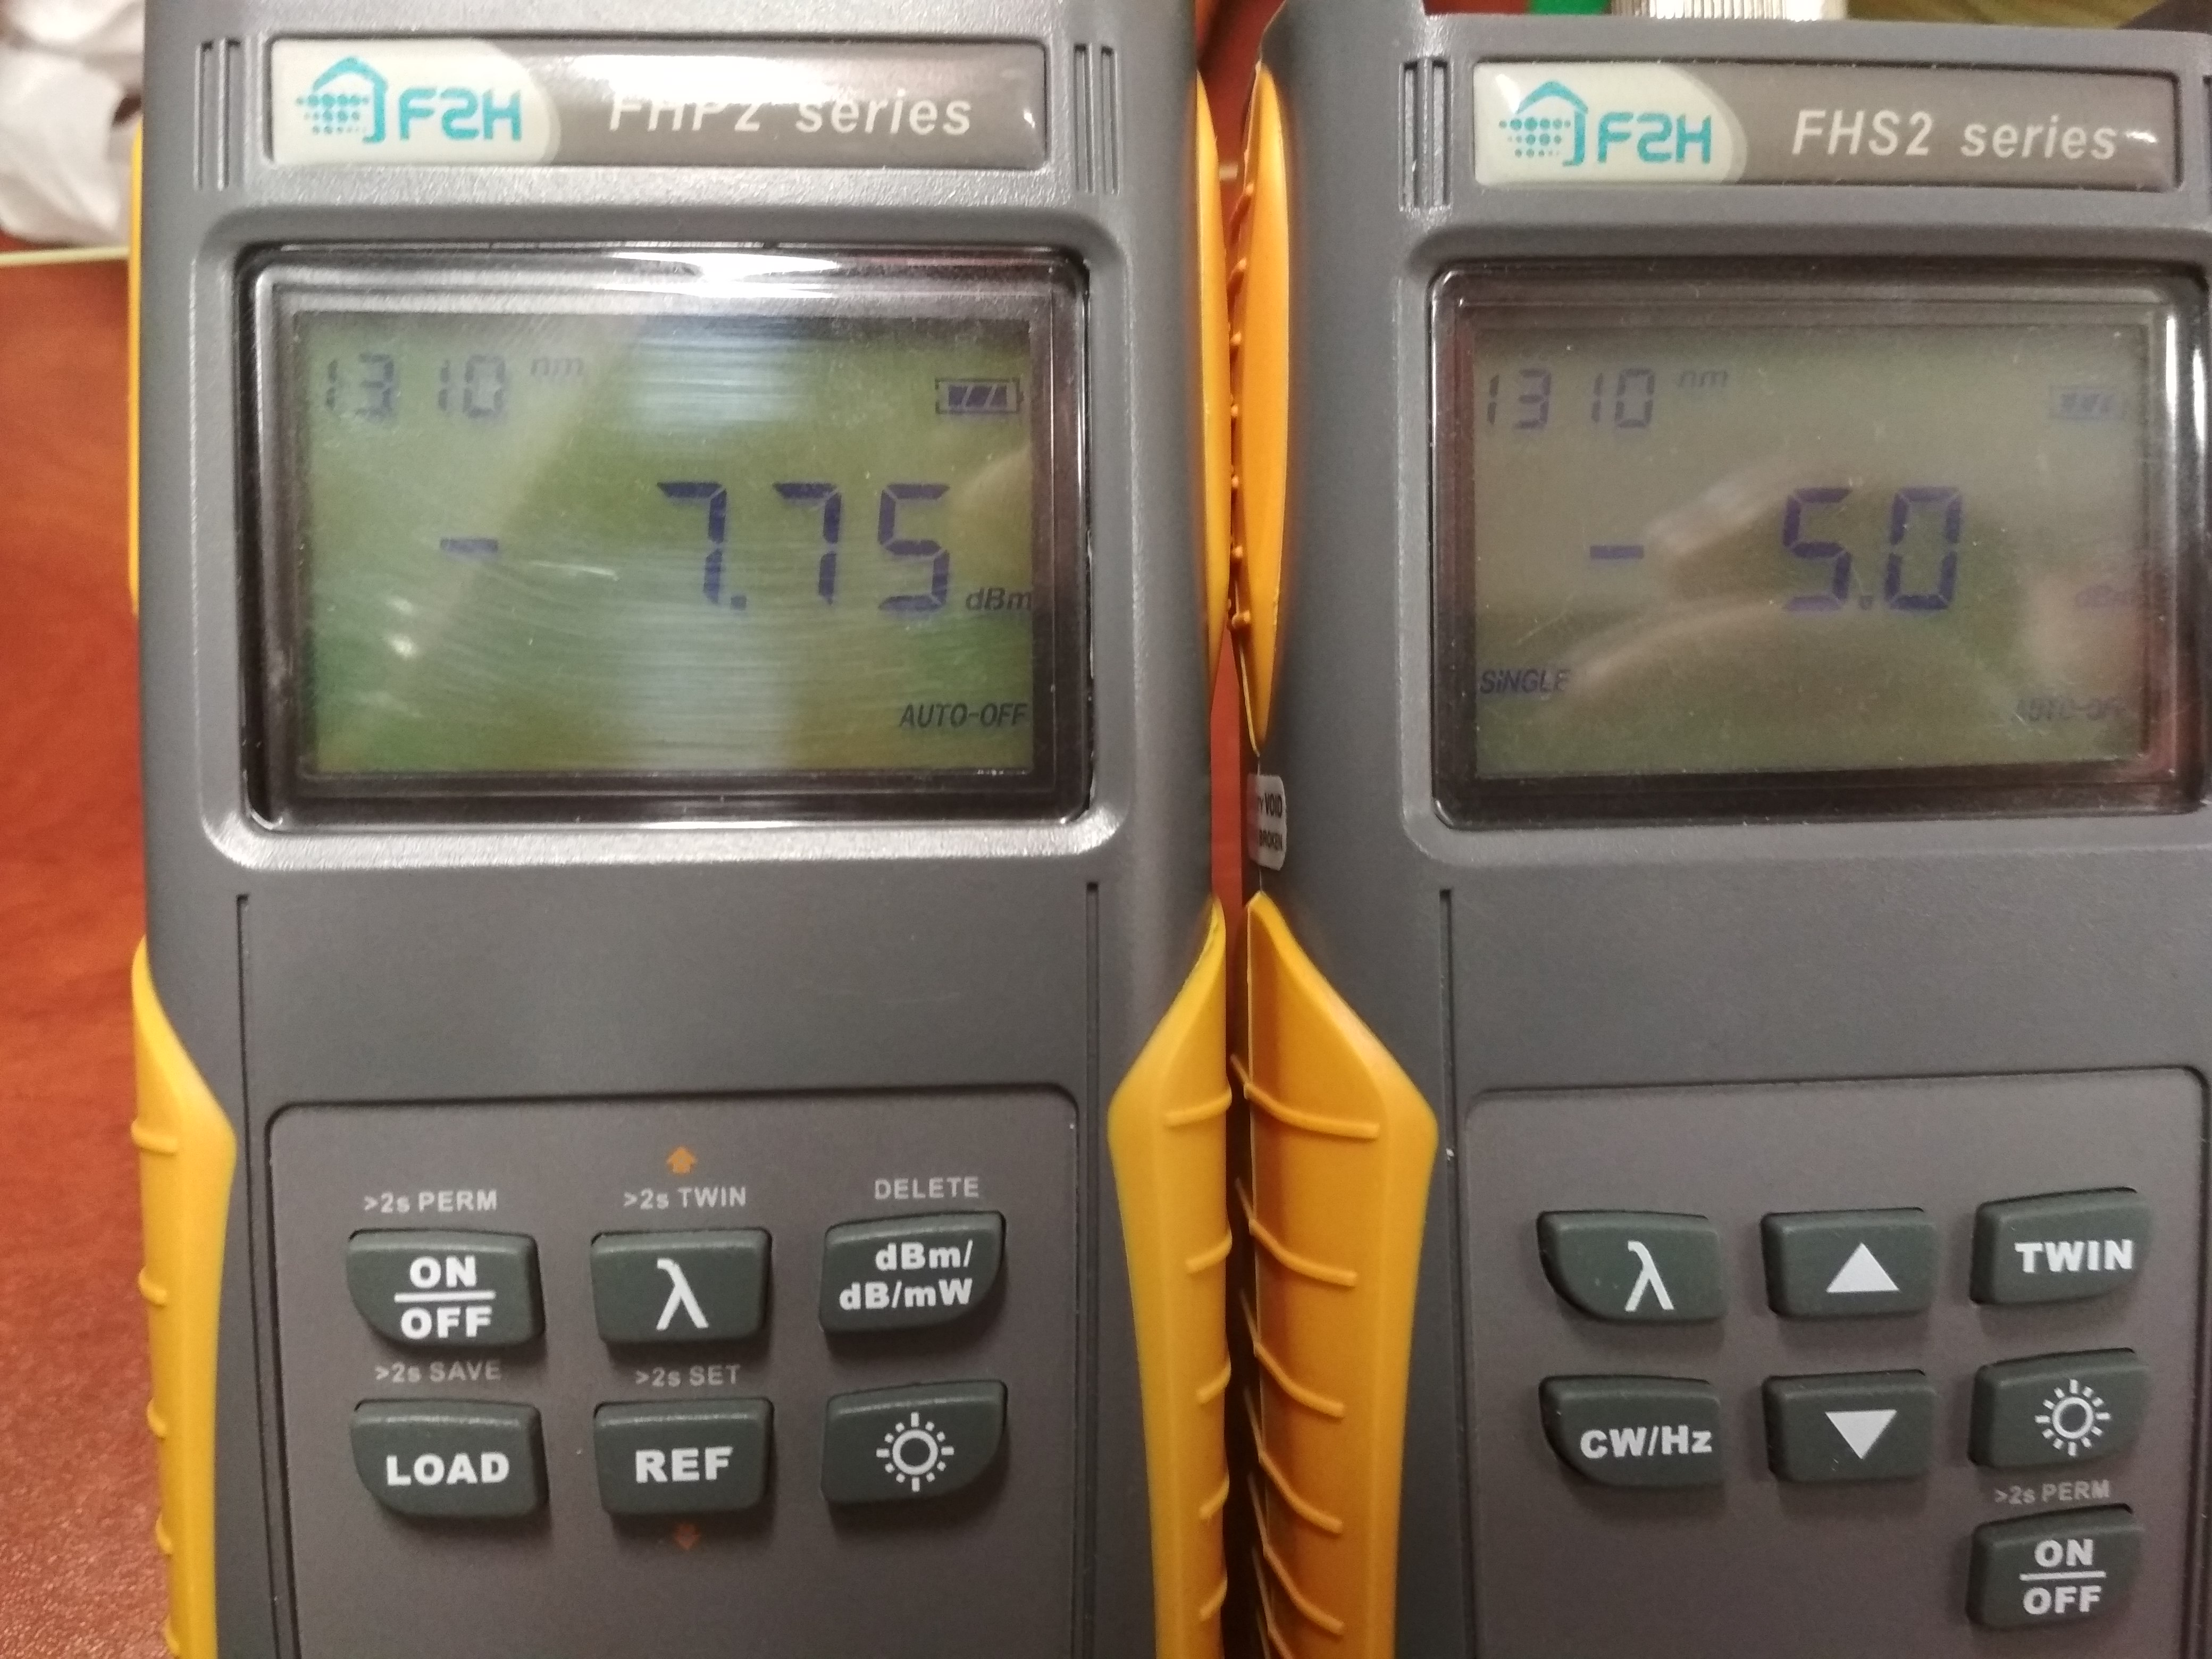
\includegraphics[scale=0.075]{f6.jpg}
\end{figure}
\clearpage
\section{Wnioski}
\begin{itemize}
\item Wykonanie prespawu w zauważalny sposób oczyściło rdzeń z zanieczyszczeń.
\item Istotnym elementem procesu jest wycentrowanie. Dzięki temu światłowód posiada odpowiednio małe straty odbiciowe w miejscu spawu, który jest wytrzymały na naprężenia. Podczas laboratorium wykorzystano dwa identyczne włókna do wykonania spawu. Jest jednak możliwość centrowania różnych włókien względem rdzenia - mniejsze odbicia i mniejsza wytrzymałość oraz względem płaszcza - większe odbicia i większa wytrzymałość.
\item Analizując rys. 5 można stwierdzić, że spaw został wykonany poprawnie i nie posiada uchybień. Podczas laboratorium został on także przeanalizowany pod innym kątem kamery, co dawało prawie identyczny obraz.
\item Rysunek 6 obrazuje intensywność światła. Wskazuje on na poprawność wykonania spawu.
\item Na podstawie odczytów z rys. 7 można określić straty L = 2.75 dB. Długość światłowodu wynosiła około 1 km, zakładamy pesymistycznie, że jego tłumienie wynosi 2 dB/km. Pozostałe 0.75 należy rozdzielić na spaw oraz złącza na wyjściu z nadajnika oraz na wejściu do odbiornika. Tłumienie złączek określa się typowo na 0.2 - 1 dB. W najbardziej pesymistycznym wypadku tłumienie spawu może więc wynosić 0.35 dB, jednak w rzeczywistości z pewnością jest mniejsze.
\item Wykonany spaw cechował się dobrą wytrzymałością, nie uległ zerwaniu przy naprężaniu.
\end{itemize}
\end{document}